ในการสร้างโมเดลปัญญาประดิษฐ์นั้นการใช้จำนวนชั้นเยอะนั้นจะทำให้ได้คุณลักษณะของข้อมูลที่ออกมาเยอะตามไปด้วย 
แต่การที่คุณลักษณะของข้อมูลเยอะไม่ได้หมายความว่าโมเดลปัญญาประดิษฐ์จะให้ประสิทธิภาพที่ดีเสมอไป ซึ่งสามารถแก้ปัญหานี้ได้โดยใช้ residual network (ResNet)\textsuperscript{\cite{he2016deep}} 
ซึ่งเป็น CNN ประเภทหนึ่ง ที่ส่วนใหญ่จะนำมาใช้กับข้อมูลที่เป็นภาพ เช่น การจดจำวัตถุ เป็นต้น โดย ResNet นี้จะสามารถทำการข้ามชั้นที่ไม่จำเป็นได้ 
การข้ามชั้นที่ไม่จำเป็นจะช่วยให้ข้อมูลที่ได้ออกมานั้นดีที่สุด

\begin{figure}[!ht]
	\centering
	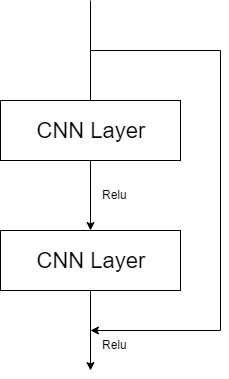
\includegraphics[width=0.5\textwidth]{chapter2/images/example_resnet.png}
		\caption{หลักการของ Residual block ของ ResNet}
    	\label{fig:ResNet}
\end{figure}

การทดลองโมเดลปัญญาประดิษฐ์ ResNet ด้วยการทำจำแนกภาพโดยใช้ชุดข้อมูลทดสอบ ImageNet ที่มีหมวดหมู่มากกว่า 1,000 หมวดหมู่
มาเทียบกับโมเดลปัญญาประดิษฐ์ทั่วไป (plain model) ที่จำนวนชั้น 18 ชั้น และ 34 ชั้น โดยโครงสร้างพื้นฐานของโมเดลปัญญาดิษฐ์ ResNet และโมเดลปัญญาประดิษฐ์ทั่วไปเหมือนกัน 
ซึ่งผลลัพธ์อัตราร้อยละของความผิดพลาดจะได้ออกมาตามตารางที่ \ref{tab: Top-1 error of ImageNet} 

\begin{table}[!ht]
	\centering
	\begin{tabular}{|c|c|c|}
		\hline
		{จำนวนชั้นของโมเดลปัญญาประดิษฐ์}&\multicolumn{2}{c|}{Training error}\\
		\cline{2-3}
		{}							& plain						& ResNet			\\
		\hline
		18							& 27.94						& 27.88				\\
		34							& 28.54						& 25.03				\\
		\hline
	\end{tabular}
	\caption{อัตราร้อยละของความผิดพลาดของชุดข้อมูลทดสอบ ImageNet}
	\label{tab: Top-1 error of ImageNet}
\end{table}

จากตาราง \ref{tab: Top-1 error of ImageNet} จะเห็นได้ว่าโมเดลปัญญาประดิษฐ์ทั่วไป 34 ชั้นมีค่าอัตราร้อยละของความผิดพลาดสูงกว่าโมเดลปัญญาประดิษฐ์ ResNet 
ได้อย่างชัดเจน ในขณะที่โมเดลปัญญาประดิษฐ์ทั่วไปจะมีอัตราร้อยละของความผิดพลาดสูงขึ้นเมื่อเทียบกันระหว่าง 18 ชั้นและ 34 ชั้น
\clearpage
ต่อมาจะนำโมเดลปัญญาประดิษฐ์ ResNet มาทดสอบกับชุดข้อมูล CIFAR-10 ซึ่งเป็นชุดข้อมูลที่มีรูปสำหรับใช้สร้างโมเดลปัญญาประดิษฐ์ 50,000 รูป รูปสำหรับทดสอบ 10,000 รูป 
และมีจำนวนหมวดหมู่ทั้งหมด 10 หมวดหมู่ โดยจะมีการออกแบบของจำนวนชั้นของโมเดลปัญญาประดิษฐ์ ResNet ตามจำนวนของชั้น convolution 
ที่มีผังคุณลักษณะเท่ากัน 6 ชั้นติดกันและการข้ามชั้นทีละ 2 ชั้น จึงทำให้ได้รูปแบบการคิดชั้นดังนี้ 6n + 2 สำหรับการทดสอบจะให้ค่า n = [3, 5, 7, 9, 200] ดังตารางต่อไปนี้

\begin{table}[!ht]
	\centering
	\begin{tabular}{|c|c|c|}
		\hline
		{โมเดลปัญญาประดิษฐ์}		  &{จำนวนชั้น}				    &{Training error}	\\
		\hline
		ResNet						& 20						& 8.75				\\
		ResNet						& 32						& 7.51				\\
		ResNet						& 44						& 7.17				\\
		ResNet						& 56						& 6.97				\\
		ResNet						& 110						& 6.43				\\
		ResNet						& 1202						& 7.93				\\
		\hline
	\end{tabular}
	\caption{ค่าความผิดพลาดที่ได้จากการทดลองจำนวนชั้นของโมเดลปัญญาประดิษฐ์ ResNet บนชุดของข้อมูล CIFAR-10}
	\label{tab: หมวดหมู่ification error}
\end{table}
จากตาราง \ref{tab: หมวดหมู่ification error} จะเห็นได้ว่าที่โมเดลปัญญาประดิษฐ์ ResNet ที่มีจำนวนชั้น 1,202 
นั้นมีค่าความผิดพลาดเกิดขึ้นมากกว่าจำนวนชั้น 110 ซึ่งอาจจะเป็นไปได้ว่าขนาดของโมเดลปัญญาประดิษฐ์ ResNet ที่มีจำนวนชั้น 1,202 
นั้นมากเกินไปสำหรับชุดข้อมูลขนาดเล็กนี้